%harihiom
\documentclass{llncs}

\usepackage[english]{babel}
%\usepackage[utf8]{inputenc}
%\usepackage{amsmath}
\usepackage{graphicx}
\usepackage{float}
%\usepackage{wrapfig}
%\usepackage{titlepic}
%\usepackage[colorinlistoftodos]{todonotes}
\usepackage{graphicx,epstopdf}
\usepackage{amsmath,amssymb,amsfonts,subfigure}
\usepackage{comment}
\usepackage{algorithm}
\usepackage{algpseudocode}
\usepackage{pifont}
\usepackage[normalem]{ulem}
\usepackage[english]{babel}
\usepackage[utf8x]{inputenc}
\usepackage{graphicx}
\usepackage{calc}
\usepackage{graphicx}
\usepackage{subfigure}
\usepackage{gensymb}
\usepackage{natbib}
\usepackage{url}
\usepackage[utf8x]{inputenc}
\usepackage{amsmath}
\usepackage{graphicx}
\graphicspath{{images/}}
\usepackage{parskip}
\usepackage{fancyhdr}
\usepackage{vmargin}
\usepackage{algorithm}
\linespread{1}
\usepackage{color}
\usepackage{cite}
\usepackage{amsmath,amssymb}
\newtheorem{claim1}{Claim}
\usepackage{algpseudocode}% http://ctan.org/pkg/algorithmicx
\usepackage[compatibility=false]{caption}% http://ctan.org/pkg/caption
\setmarginsrb{3 cm}{2.5 cm}{3 cm}{2.5 cm}{1 cm}{1.5 cm}{1 cm}{1.5 cm}

%\newtheorem{theorem}{Theorem}
%\newtheorem{lemma}{Lemma}

\title{Lecture - 4}
\author{Wednesday, 3 August 2016 (14:25- 15:15)}
\institute{\textbf{German Tank Problem}}

\begin{document}
\maketitle
\vspace{1cm}
\section{German Tank Problem}

In the second world war, Allies wanted to estimate the extent of German production in terms of the total number of tanks possessed by Germany. What the Allies had at hand were some of the German tanks they have captured. There was a unique serial number which was assigned to very German tank. This serial numbers were consecutive. Hence, the Allied had some of these numbers now, written on the tanks they have captured. With the help of this data, it was challenging to predict what is the actual number of tanks Germans had produced till then. This is shown in Figure \ref{tanks}\\ 
\begin{figure}[h!]
\centering
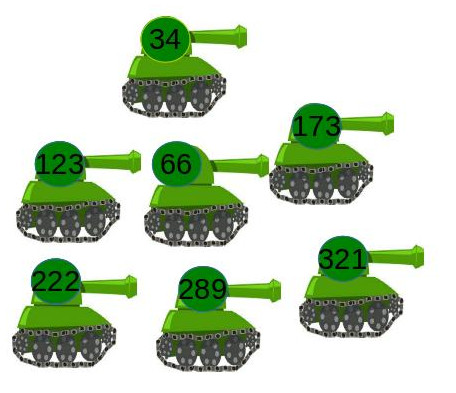
\includegraphics[width=0.6\textwidth]{german_tank.jpg}
\caption{A hypothetical example of the tanks captured by the Allies in the second world war}
\label{tanks}
\end{figure}
The figure shows the numbers of the some of the German tanks that have been captured. Can you predict the total number of tanks German army has produced by looking at this number? \\

The Allies outsourced this problem to two kinds of people -i) The statisticians and ii) Gathered intelligent mass. Whom do you think won? According to the empirical data evidence by Wikipedia, in August 1942, the statisticians predicted 327 tanks, intelligent mass predicted 1550 tanks and according to the German records, the actual number of tanks were 342. So, the statistical theory won. Today, we are going to delve deep in this statistical method used in the second world war. \\

To better get a picture of the problem, assume a college where each student is given a unique serial number from 1 to n ( where n is total number of students ). The newly hired gatekeeper is observing the passing by students and asking them their serial numbers (The students are assumed to be honest). By looking at $k$ students, can the gatekeeper approximate the total number of students in the institute. Can you see this problem being nothing but another way of writing the German Tank Problem. \\

\textbf{\large Formal Definition of the problem}:\\
$S$ is a set of numbers from $1$ to $n$. We are given a subset of $S$, say $T$ of k numbers. $T=$\{$a_1,a_2,a_3,.....a_k$\} such that $a_i<a_{i+1}$ (We can arrange the given set $T$ in a sorted order). What is the best value of $n$ one can predict from here? For sure, the value of $n$ is definitely larger than $a_k$, since $a_k$ is one of the numbers from $1$ to $n$. 
Now the question can be asked: Is $a_k$ a good estimate of $n$?\\

To answer this question, we find out the expected value of $a_k$. $a_k$ is a random variable, which can take values from $k$ to $n$ (Why not from $1$ to $n$\footnote{Since, $a_k$ is the highest value among the sampled $k$ numbers, it can never be less than $k$. In the worst case, where $a_k$ is minimum, $T$ has to be $\{1,2,3,.....,k\}$}? ). \\

So, $E[a_k] = \sum_{\alpha=k}^{n} \alpha \times pr(a_k= \alpha)$\footnote{pr() refers to probability() in the given formula.}  \hspace{3cm} ...... (1) \\

What is left now is to calculate $Pr(a_k=\alpha)$. Consider Figure \ref{ak}. For $\alpha$ to be the highest element is the chosen set $T$ of $k$ elements, the remaining $k-1$ elements should be less than $\alpha$. There are total $\binom{\alpha-1} {k-1}$ ways from set $S$ in which these $k-1$ elements can be chosen from the $\alpha - 1$ elements. The total number of ways in which $k$ elements of $T$ can be chosen from the $n$ elements of $S$ are $\binom {n} {k}$.
\begin{figure}[h!]
\centering
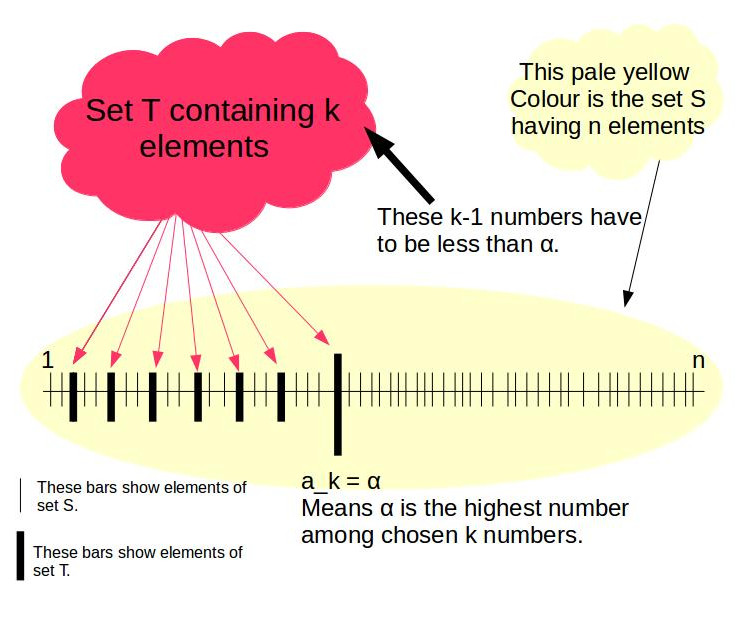
\includegraphics[width=\textwidth]{ak.jpg}
\caption{Finding pr ($a_k=\alpha$)}
\label{ak}
\end{figure}

\begin{center}
Pr\{ $a_k = \alpha $ \}= $\frac{ \binom {\alpha -1} {k-1} }{\binom {n} {k}}$\\
\end{center}

From (1)\\
\begin{center}
E\lbrack $a_k$ \rbrack=$ \sum_{\alpha=k}^n \alpha$
$\frac{ \binom {\alpha -1} {k-1} }{\binom {n} {k}}$
\end{center}

\begin{center}
= $ \frac{1}{\binom{n}{k}} \sum_{\alpha=k}^n \alpha  \frac{(\alpha -1)!} {(k-1)! \times (\alpha -k)!}$
\end{center}

Multiplying numerator and denominator by $k$ \\

\begin{center}
$E[a_k]$= $ \frac{1}{\binom{n}{k}} \sum_{\alpha=k}^n \alpha \times k \frac{(\alpha -1)!} {k \times (k-1)! \times (\alpha -k)!}$
\end{center}

or\\

\begin{center}
E\lbrack $a_k$ \rbrack=$\frac{k}{\binom {n} {k}} \sum_{\alpha=k}^n \frac {\alpha !}{(\alpha - k)!k!}$\\
\end{center}

or \\

\begin{center}

E\lbrack $a_k$ \rbrack=$\frac{k}{\binom {n} {k}} \sum_{\alpha=k}^n \binom {\alpha} {k}$ \hspace{1cm} .. (2)\\
\end{center}

\begin{center}
$\frac{k}{\binom {n} {k}} \times \binom {n+1}{k+1}$ \hspace{1cm} .. (3)\\
\end{center}

To understand the transition from (2) to (3), i.e. how $ \sum_{\alpha=k}^n \binom{\alpha}{k} $ = $ \binom {n+1}{k+1}$ please refer Appendix. \\
Simplifying further, we get\\

\begin{center}
E\lbrack $a_k$ \rbrack=$\frac{k}{k+1}\times  (n+1)$\\
\end{center}
From the above expression $n$ can be derived in terms of $E[a_k]$.\\

The value of $a_k$ varies every time  when you do the experiment. We represent this value by $\hat{a_k}$. How do we ensure that $\hat{a_k}$ can be used to find a very good estimate of $n$?\\

We calculate $n$ as follows.\\

$n= \frac{k+1}{k} \times \hat{a_k}-1$\\

 E\lbrack $ \frac{k+1}{k} \times a_k  - 1 $ \rbrack 
 = $\frac{k+1}{k}   E(a_k) - E(1)$ = $n$ \\

Hence, the formula gives us a very good estimate of $n$.\\

\subsection{Verification by an interesting activity done in the class}

The students were asked to install an application which generated random numbers from a given range of integers. We chose $n=1000$. 

\begin{enumerate}
\item 10 students was asked to generate\footnote{Please note that there is no relation between taking both the number of students and the number of randomly generated values as 10. It is a coincidence.} 10 random numbers from the range of 1 to 1000, and report the maximum value. Please note that each individual value reported by an student acts as a distinct $\hat{a_k}.$
\item The set of $\hat{a_k}$ values =\{984, 915, 819, 896, 835, 931, 955, 975, 946, 939\}. 
\item Next, we used the formula to find $n$, given as $n= \frac{k+1}{k} \times \hat{a_k}-1$.
\item The set of corresponding values of $n$  was observed to be \{1081, 1005, 899, 984, 917, 1023, 1049, 1071, 1039, 1031\}\\
 \end{enumerate}

\begin{itemize}
\item Average sum of these values=$1009.90$. There is an error of $9.9$. This error might have occurred because of less number of samples. As we increase the sample size $k$, error diminishes.\\

How many numbers should we take here to get n=1000 exactly? Can we compute an upper bound for this?\\
This is similar to the question- \\
 Let's say there is a biased coin with probability of head ($\frac{1}{2} -\epsilon$) and tail ($\frac{1}{2} +\epsilon$). Now how many times should I toss the coin to get 50 heads?\\
Such kinds of problems can be solved using Chernoff bounds, which we will discuss in the upcoming lectures. 
\item The expected value of $n$ is very close to the actual value of $n$, but there is a large standard deviation between the $n$ values for different experiments.\\

For the distribution of value of ${a_k}$ , it can be proven that,
\begin{center}
Variance=$\frac{n^2}{k^2},\sigma=\frac{n}{k}$ \\
The above is left as a tutorial question to be proven.

\end{center}
\end{itemize}

\vspace{2cm}

\appendix
\begin{center}
\textbf{\huge{Appendix}}
\end{center}
\section{ Proof for $ \sum_{\alpha=k}^n \binom{\alpha}{k} $ = $ \binom {n+1}{k+1}$}
Proof:\\

$\binom{n}{k}\ =\ \binom{n-1}{k-1} + \binom{n-1}{k}$\\

Consider the above as finding the number of ways of choosing $k$ people out of $n$ people. Assume,  there is a person John in this crowd of $n$ people. \\

\textbf{Total number of ways in which $k$ people can be chosen = Number of ways where John is chosen + Number of ways where John is not chosen.} \\

\textbf{If John is already chosen}, then the remaining $k-1$ people can be chosen in $\binom {n-1}{k-1}$ ways. \\

\textbf{If John is not chosen}, then the $k$ people have to be chosen from $n-1$ people, which can be done in $\binom{n-1}{k}$ ways. \\

From the above 3 statements \\

$\binom{n}{k} = \binom{n-1}{k-1} + \binom{n-1}{k}$\\

$= \binom{n-1}{k-1} + \binom{n-2}{k-1} + \binom{n-3}{k}$  \hspace{1cm} ,by recursive application of the same formula\\

$= \binom{n-1}{k-1} + \binom{n-2}{k-1} + \binom{n-3}{k-1} + ..... + \binom{n-(n-k)}{k}$  \\

Notice that the last term in the above expression is nothing but $\binom{k}{k}$, which can be further expanded to one more step as follows : \\

$= \binom{n-1}{k-1} + \binom{n-2}{k-1} + \binom{n-3}{k-1} + ..... + \binom{n-(n-k)}{k-1} + \binom{n-(n-k+1)}{k-1}$  \\

We know that the expression can not be expanded more, because the last term is $\binom{k-1}{k-1}$. On further expansion, it becomes $\binom{k-2}{k-1}$, which is not defined. So the series end here. So, \\

$\binom{n}{k}\ = \binom{n-1}{k-1} + \binom{n-2}{k-1} + \binom{n-3}{k-1} + ..... + \binom{n-(n-k)}{k-1} + \binom{n-(n-k+1)}{k-1}$ \hspace{1cm} \\


$\binom{n}{k}\ = \sum_{\alpha=1}^{n-k+1} \binom{n-\alpha}{k-1} \hspace{1cm} ..... (4) $  \\

Let us now look at our expression\\

$\sum_{\alpha=k}^n \binom{\alpha}{k}$\\

= $\binom{k}{k} + \binom{k+1}{k} + ..... + \binom{n-1}{k} + \binom{n}{k}$\\

= $\binom{n}{k}+ \binom{n-1}{k} + .....  + \binom{k+1}{k} + \binom{k}{k} $\\ 

=  $\binom{(n+1)-1}{(k+1)-1}+ \binom{(n+1)-2}{(k+1)-1} + .....  + \binom{(n+1)-(n-k)}{(k+1)-1} + \binom{(n+1)-(n-k+1)}{(k+1)-1} $\hspace{1cm} ... (5)\\

= $\sum_{\alpha=1}^{n-k+1} \binom{(n+1)-\alpha}{(k+1)-1}$\\

It can be seen that the equations (4) and (5) are same except for $n$ has become $n+1$ and $k$ has become $k+1$. \\
Hence, \\

$\sum_{\alpha=k}^n \binom{\alpha}{k}$= $\binom{n+1}{k+1}$\\
\[
 \boxed{\sum_{\alpha=k}^n \binom{\alpha}{k}= \binom{n+1}{k+1}}
 \]


\end{document}